\documentclass[hidelinks, paper=a4, fontsize=13pt]{report}
\usepackage{graphicx}
\usepackage[utf8]{inputenc}
\usepackage{color}
\usepackage{textcomp}
\usepackage{charter}
\usepackage[T1]{fontenc}
\usepackage[top=1in, bottom=1in, left=0.7in, right=0.7in]{geometry}
\usepackage[french]{babel}
\usepackage{caption}
%\usepackage{titlesec}
\usepackage[table,xcdraw]{xcolor}
\usepackage{pdfpages}
\usepackage{sectsty} 
\allsectionsfont{\normalfont\scshape}
\usepackage{array}
\usepackage{hyperref}
\hypersetup{colorlinks=false,linktoc=all}
\usepackage{fancyhdr} 
\pagestyle{fancy} 
\fancyhead{} 
\fancyfoot[L]{24 heures de l'INSA - Guide d'accès secours - 2018} 
\fancyfoot[C]{}
\fancyfoot[R]{\thepage}
\renewcommand{\headrulewidth}{0pt}
\renewcommand{\footrulewidth}{0pt}
\setlength{\headheight}{13.6pt}
\setcounter{secnumdepth}{9}
\setlength\parindent{0pt}
\renewcommand{\thechapter}{\Roman{chapter})}
\renewcommand{\thesection}{\arabic{section}} 


\begin{document}

\begin{center}
	\rule[0.5ex]{\linewidth}{2pt}\vspace*{-\baselineskip}\vspace*{3.2pt}
	\rule[0.5ex]{\linewidth}{1pt}\\[\baselineskip]
	\huge \textbf{GUIDE D'ACCÈS SECOURS\\24 heures de l'INSA - 2018} \\[4mm]
	{\Large \textit{18, 19 et 20 mai 2018}}\\
	\rule[0.5ex]{\linewidth}{1pt}\vspace*{-\baselineskip}\vspace{3.2pt}
	\rule[0.5ex]{\linewidth}{2pt}\\
	\vspace{30mm}
	
\includegraphics[scale=2]{images/logo24h.jpg}\\
	
	\vspace{50mm}

\end{center}
	\begin{flushright}
		{\large\textsc{26 avril 2018}}
\end{flushright}

\chapter*{Contacts}

\textbf{1. PC sécurité}\\
Adresse : Bibliothèque Marie Curie, avenue Jean Capelle Ouest, INSA LYON\\
Ligne principale : \textbf{04 28 29 63 82}\\
Ligne secondaire : \textbf{04 72 43 70 70}\\

\textbf{2. Responsables sécurité}\\
Arthur Saunier (président) : \textbf{06 25 53 25 79}\\
Valentin Godrie : \textbf{07 52 62 04 69}\\
Léo Mouyna : \textbf{06 24 30 26 53}\\
\\

\textbf{3. DPS – Croix Rouge}\\
Responsable de dispositif, Loïc Morcel : \textbf{06 83 26 24 01}\\\\

\textbf{4. PCO (Poste de Commandement Opérationnel}\\
Adresse : Bibliothèque Marie Curie, avenue Jean Capelle Ouest, INSA LYON\\
\textit{Ce PC n’est armé qu'en cas de déclenchement du plan d'évacuation de niveau 3 ou du plan NOVI.\\\\
}Lignes d’urgence : 			\textbf{04 72 43 72 01   à 	04 72 43 72 04}\\
Fax : 					\textbf{04 72 43 72 05}\\

\textbf{5. Société de sécurité}\\
Responsable STAFF Sécurité, Jean-Christophe Bel : \textbf{06 98 16 40 50}\\


\section{Zone ERP}
	
	\begin{center}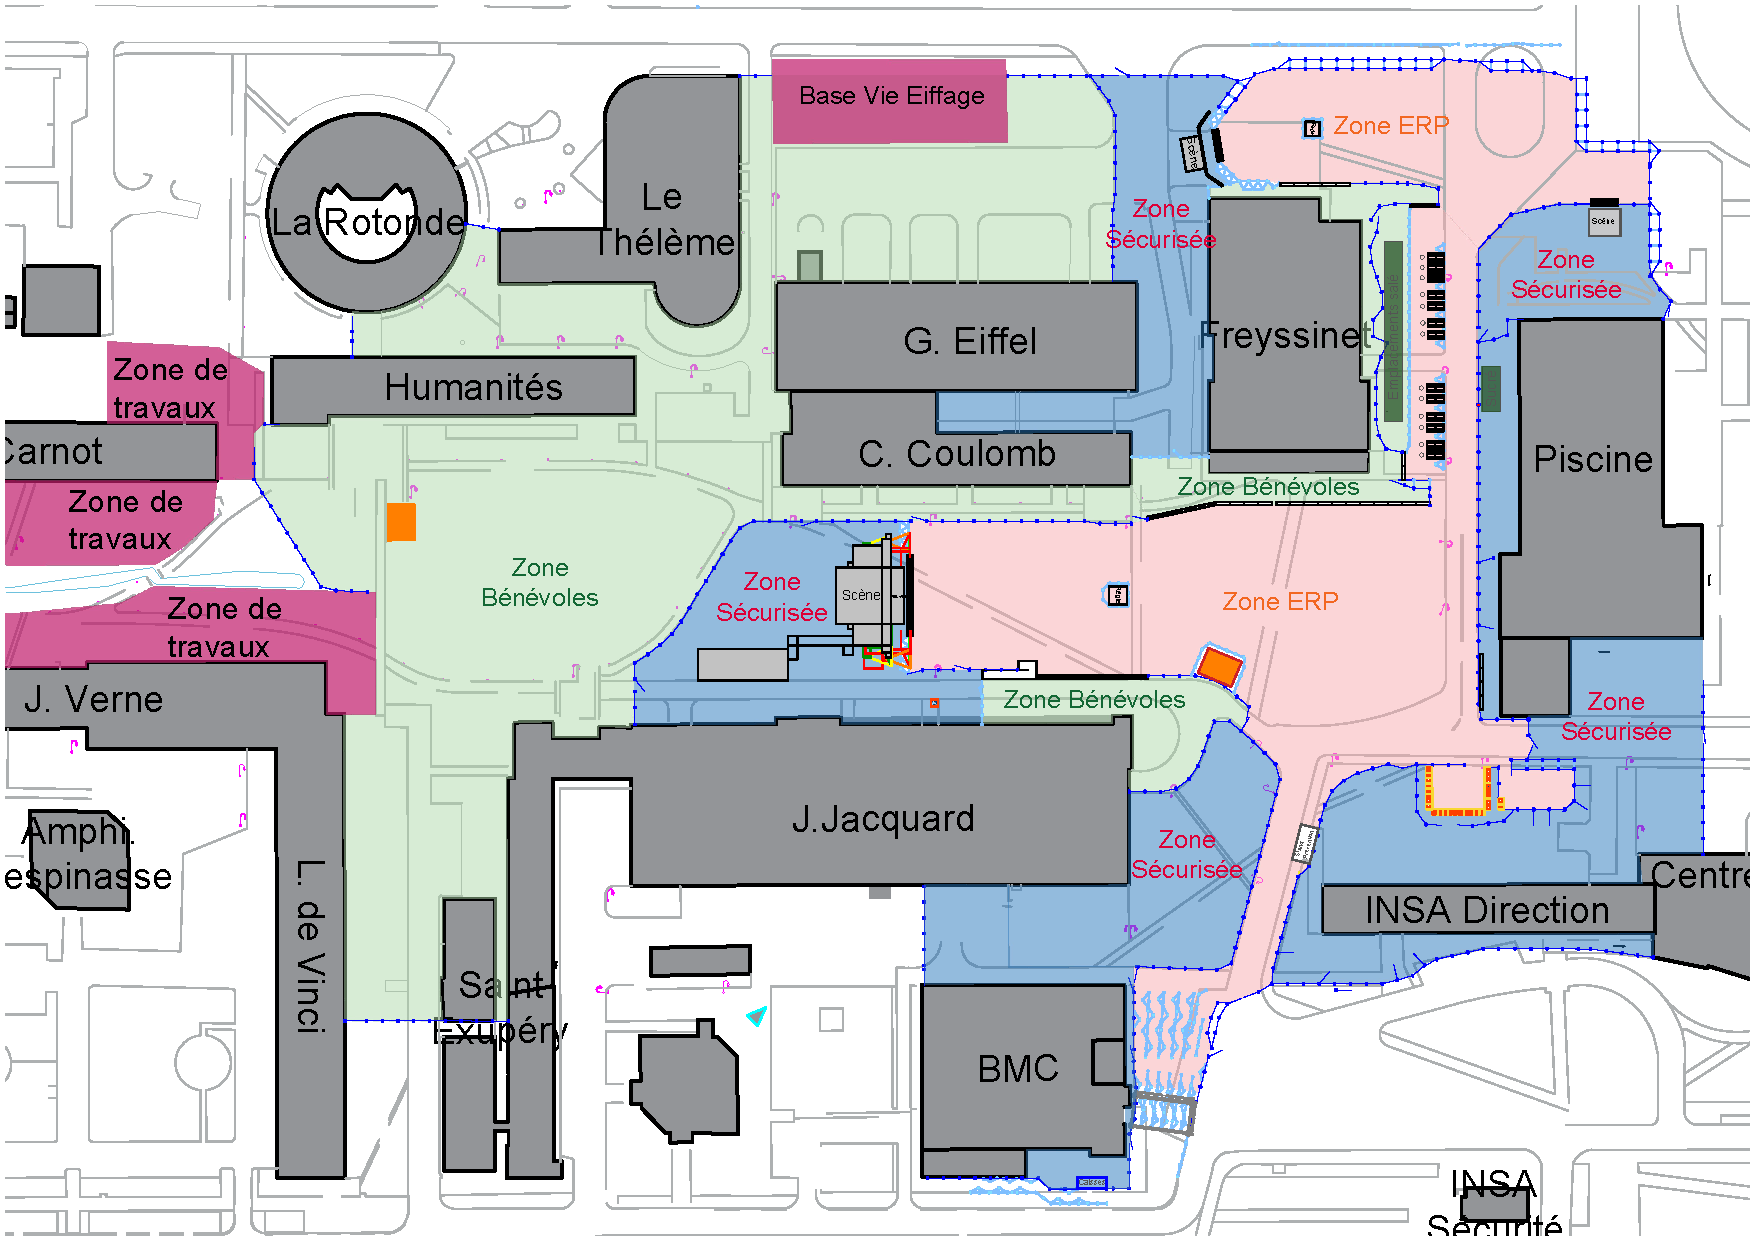
\includegraphics[width=.95\textheight,angle=90]{Exports/Plan_24h_44eme-Plan_ERP}\end{center}
	

\section{Accès Pompiers}
	\begin{center}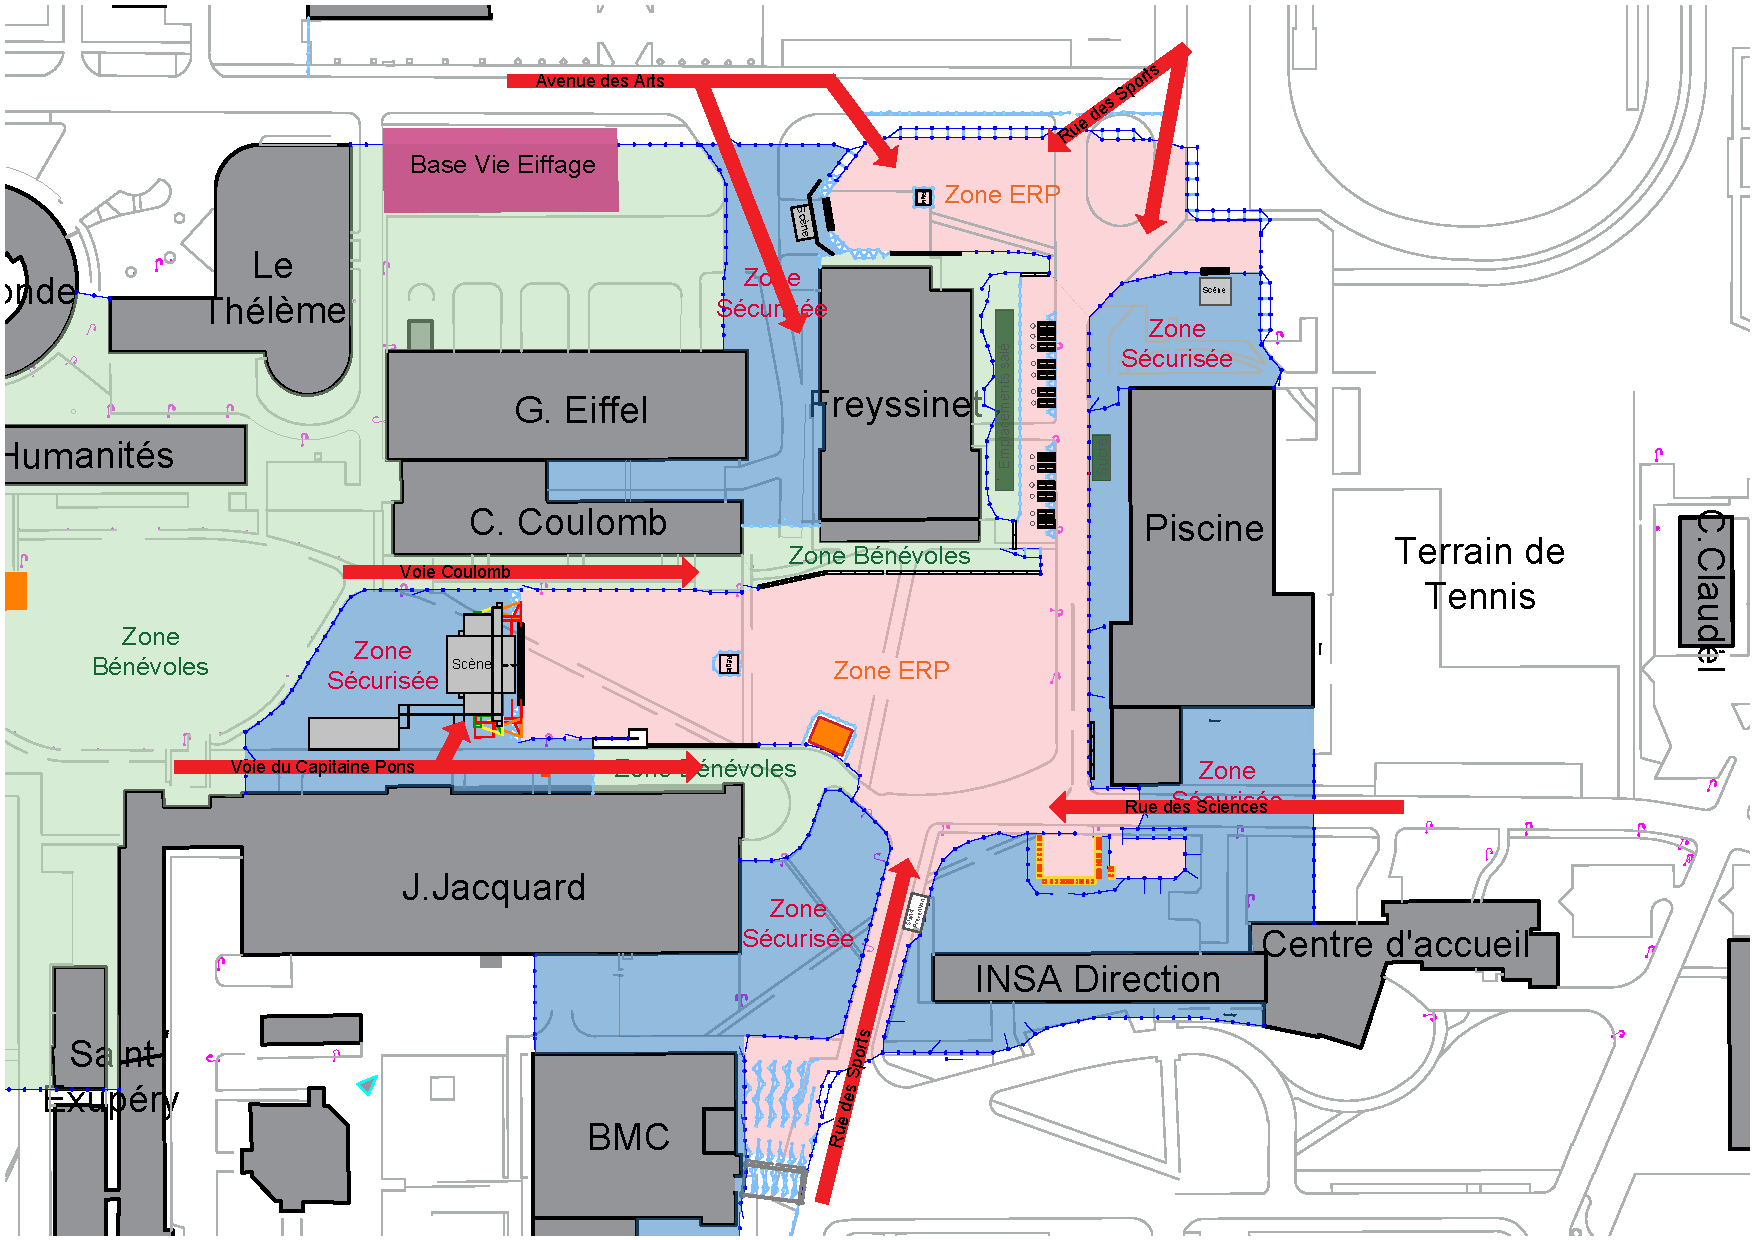
\includegraphics[width=.95\textheight,angle=90]{Exports/Plan_24h_44eme-Acces_Pompiers}\end{center}


\section{Evacuation}
	\begin{center}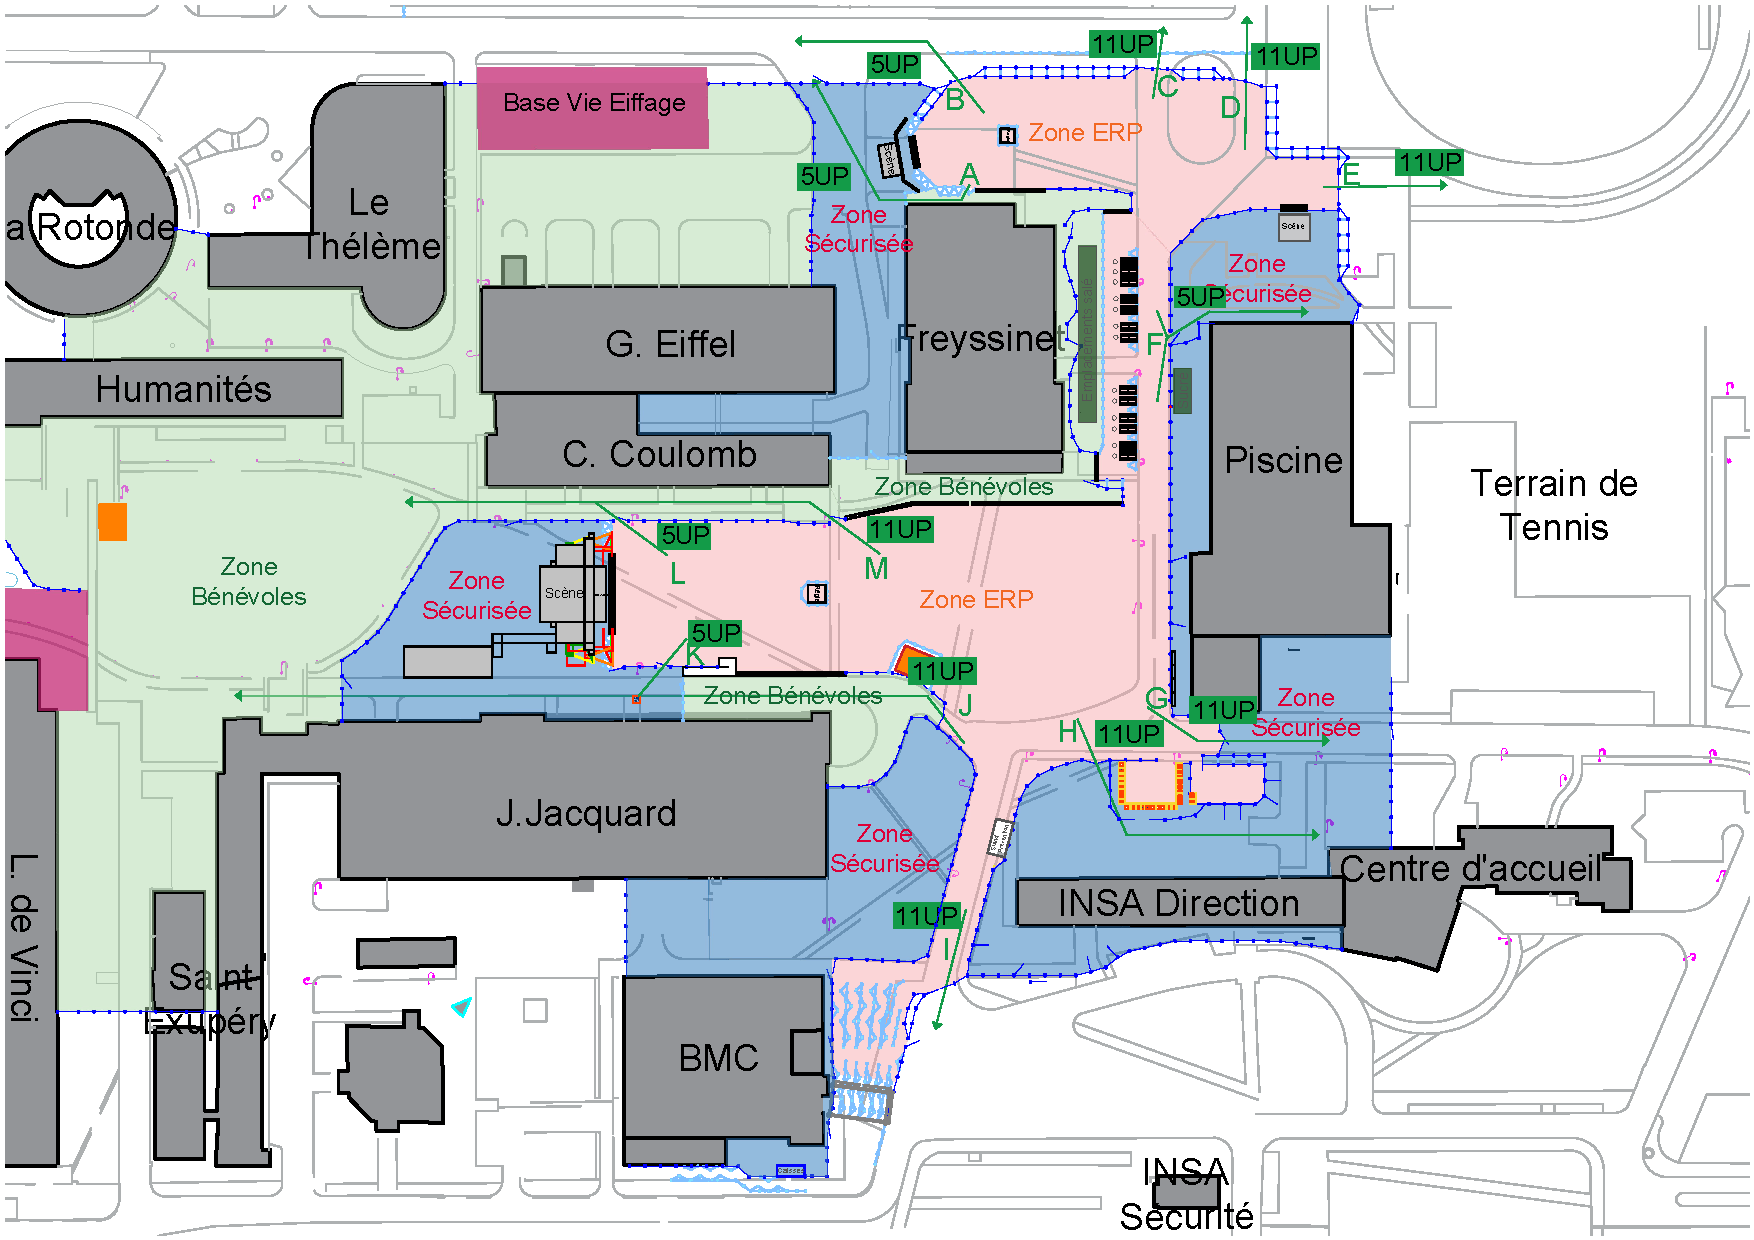
\includegraphics[width=.95\textheight,angle=90]{Exports/Plan_24h_44eme-IS}\end{center}


\section{Emplacements des PMA potentiels et du PCO}
	\begin{center}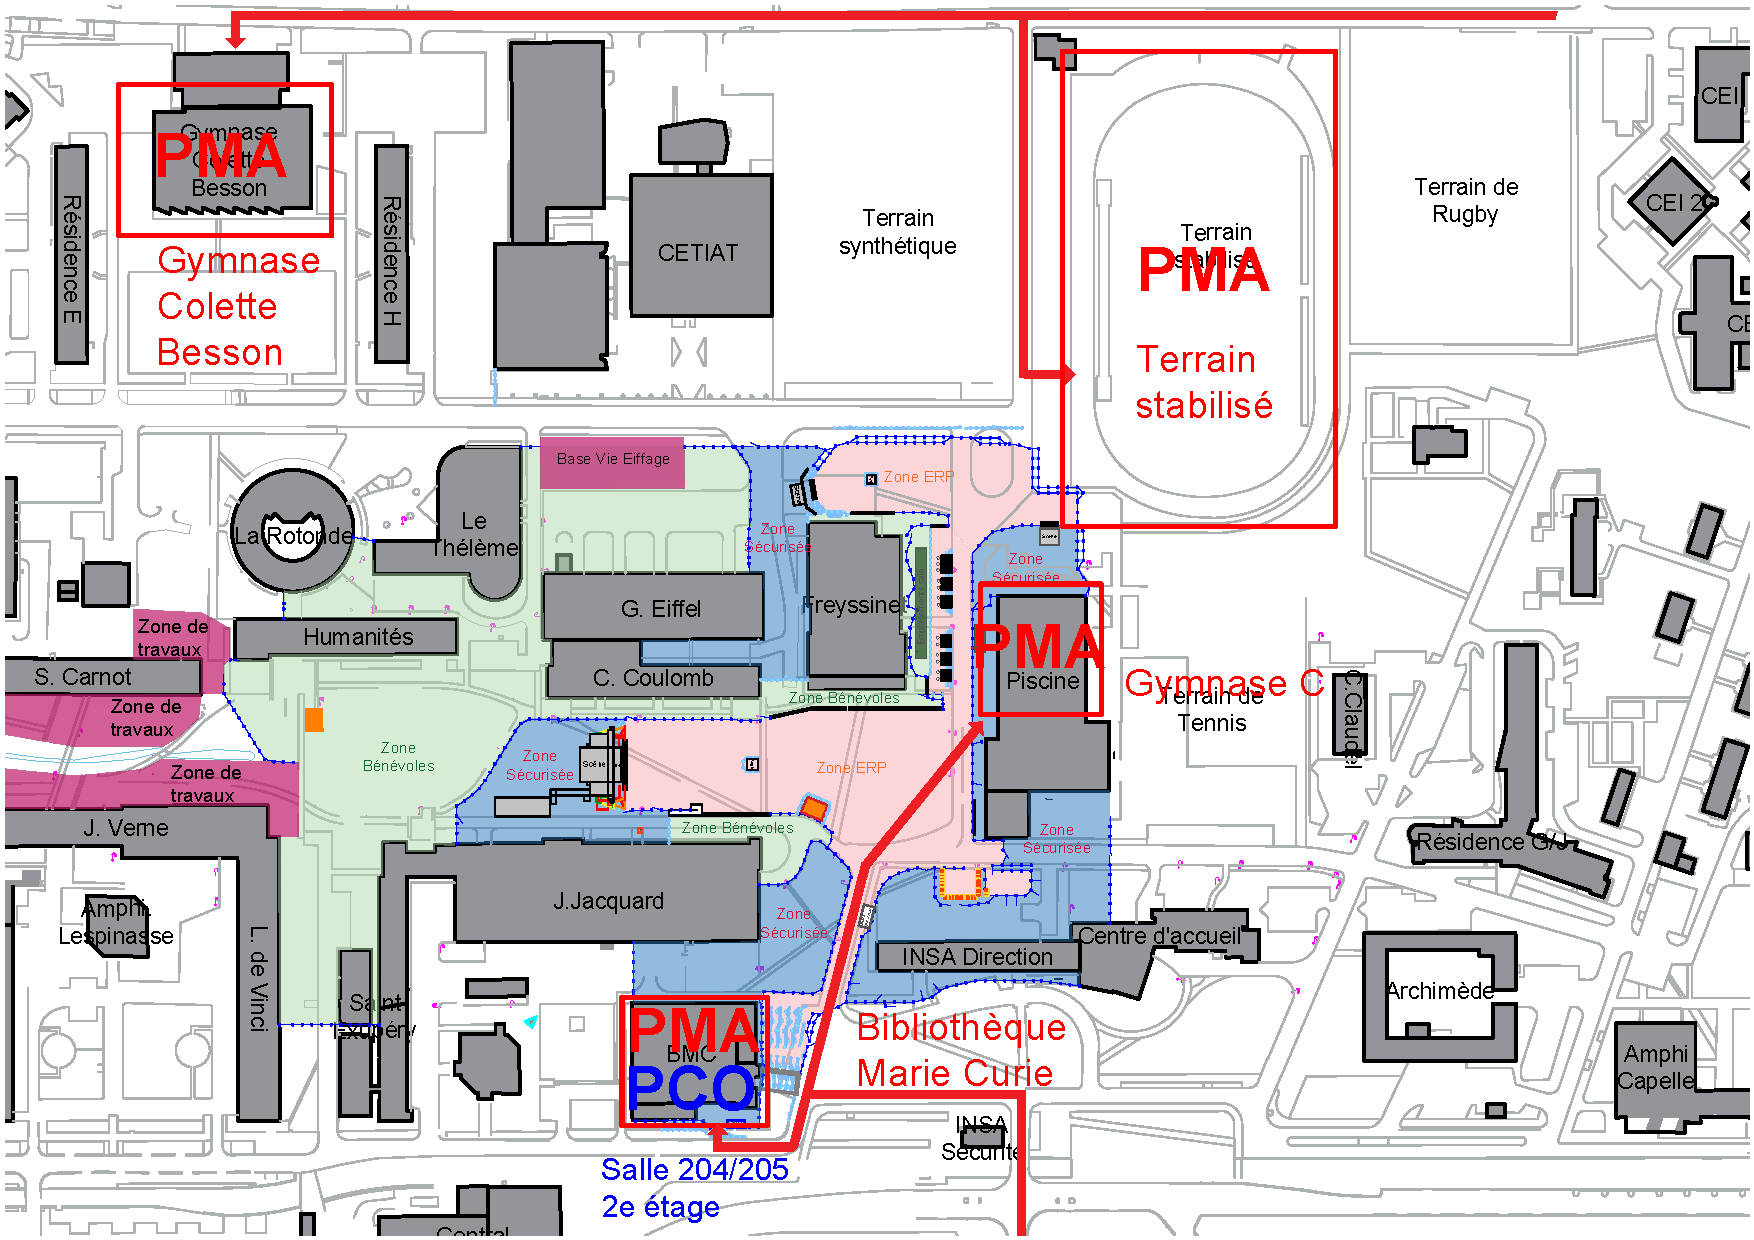
\includegraphics[width=.95\textheight,angle=90]{Exports/Plan_24h_44eme-PCO_PMA}\end{center}


\section{Circuit des courses}
	\begin{center}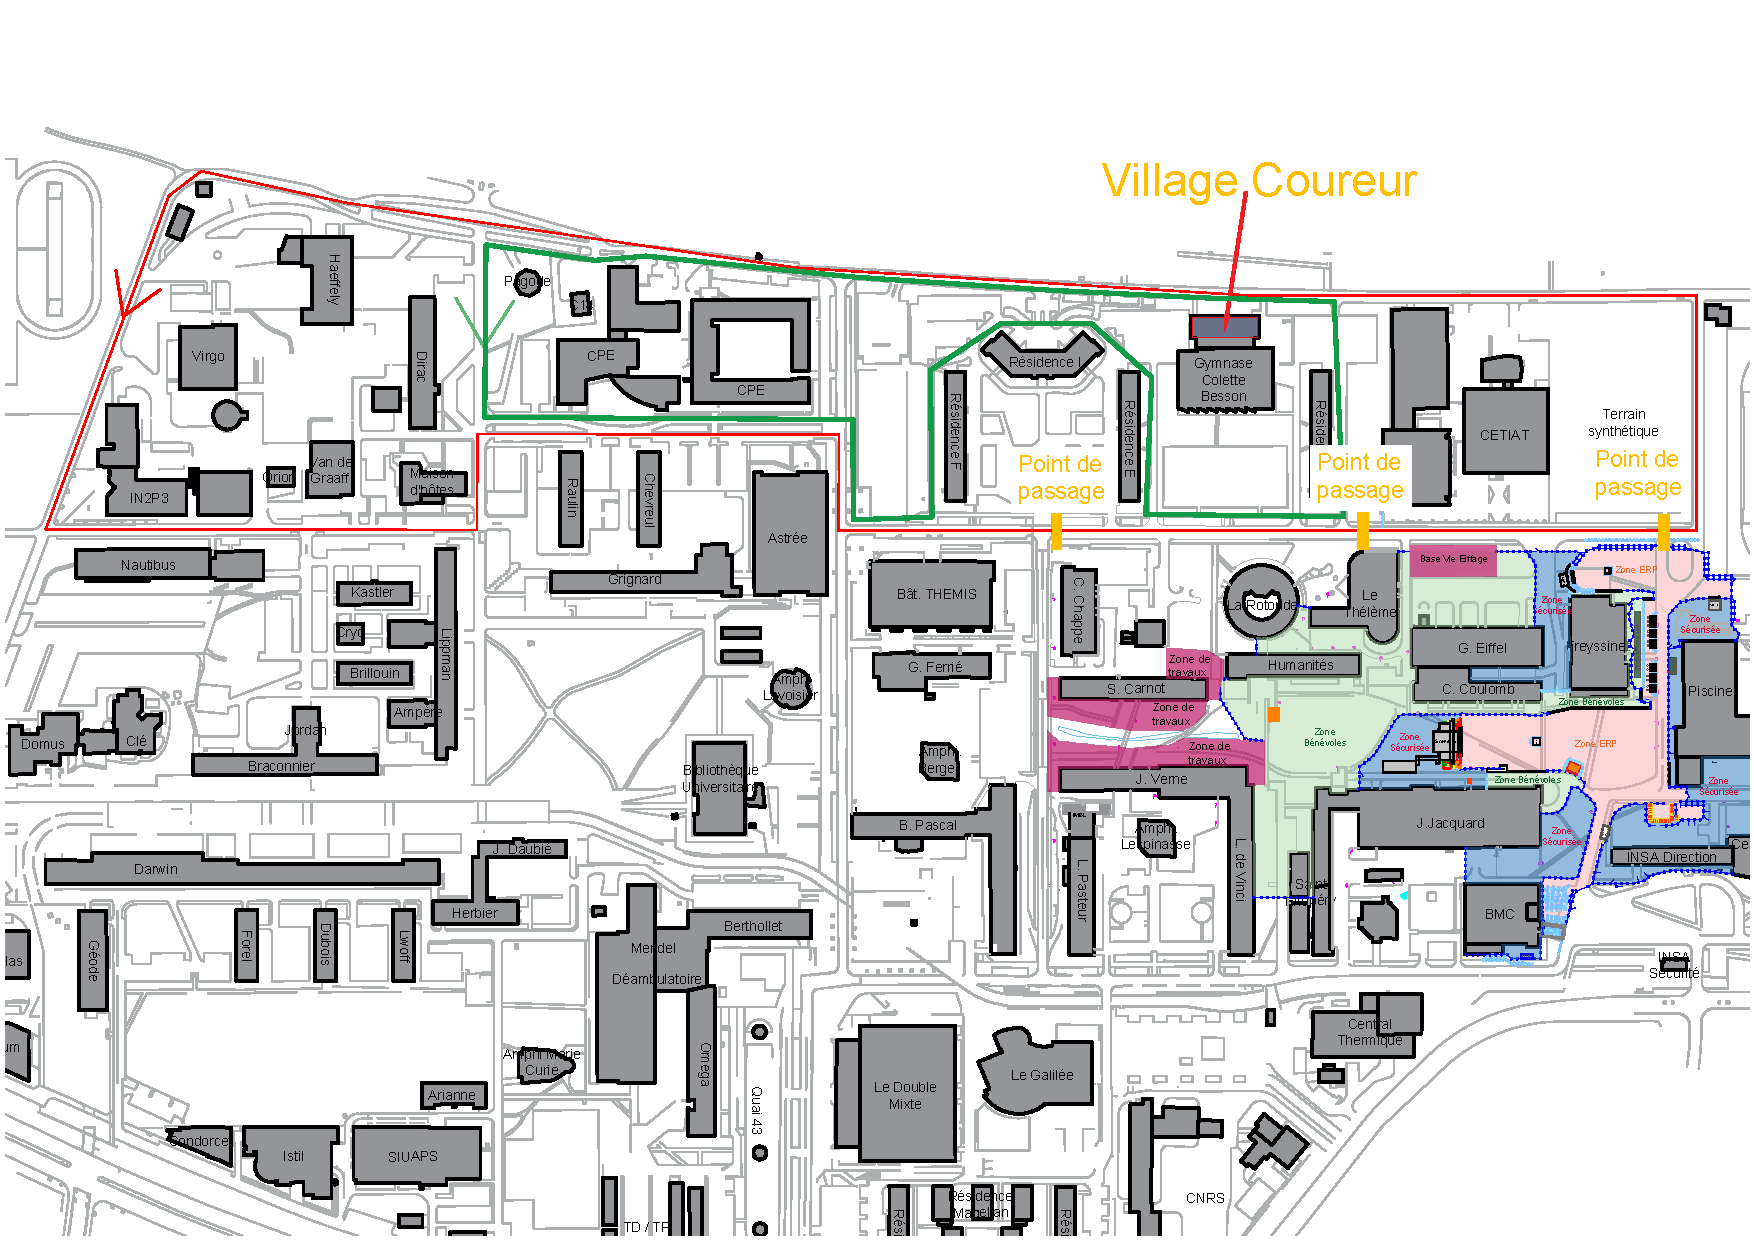
\includegraphics[width=.95\textheight, angle=90]{Exports/Plan_24h_44eme-Parcours_courses}\end{center}


\section{Accès au Campus}
Sauf mention contraire : Accès par le PS4, au 20 Avenue Albert Einstein\\
L'accès par le PS3 et le PS6 est \textbf{impossible} pour tout véhicule, \textbf{y compris les véhicules de secours} (blocs béton).
	\begin{center}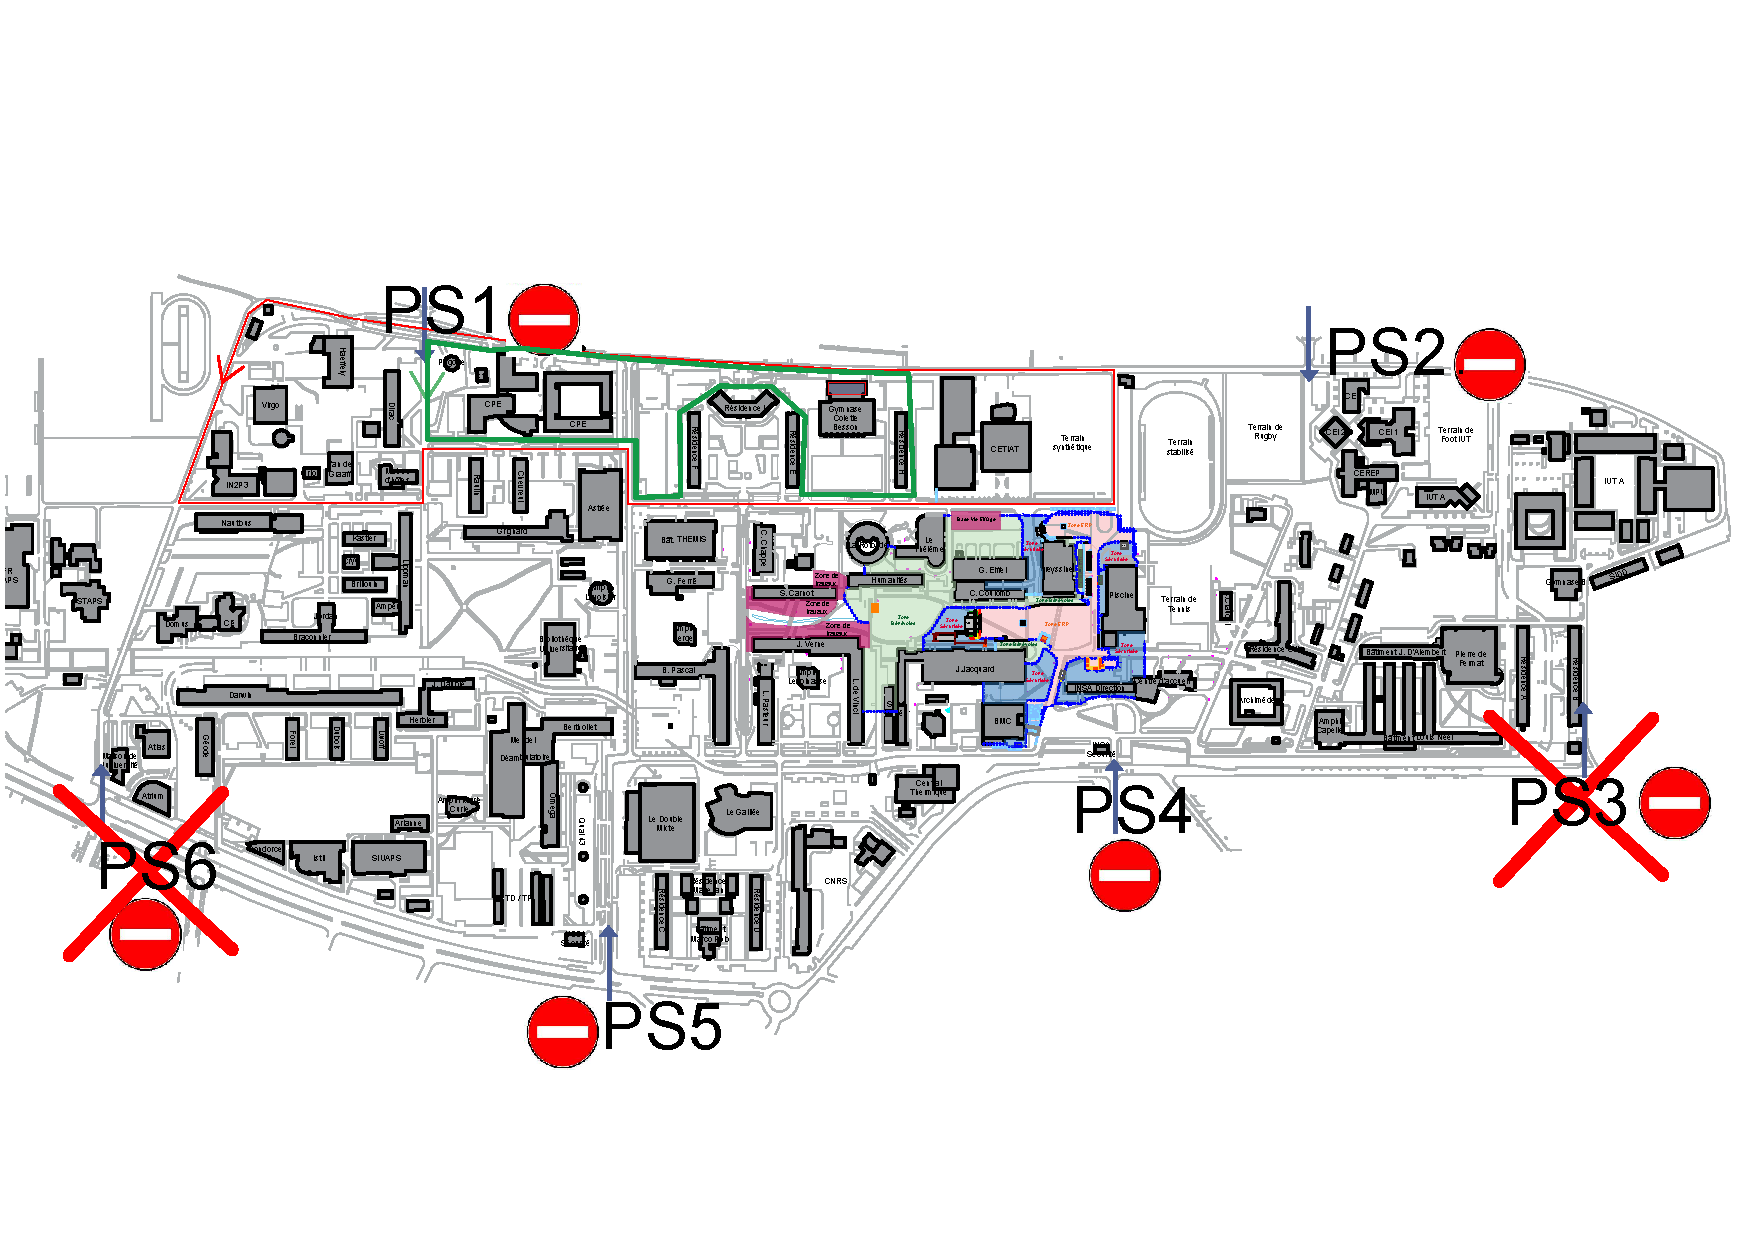
\includegraphics[width=.9\textheight, angle=90]{Exports/Plan_24h_44eme-Points_Secu}\end{center}

\section{Second périmètre de sécurtié}
	\begin{center}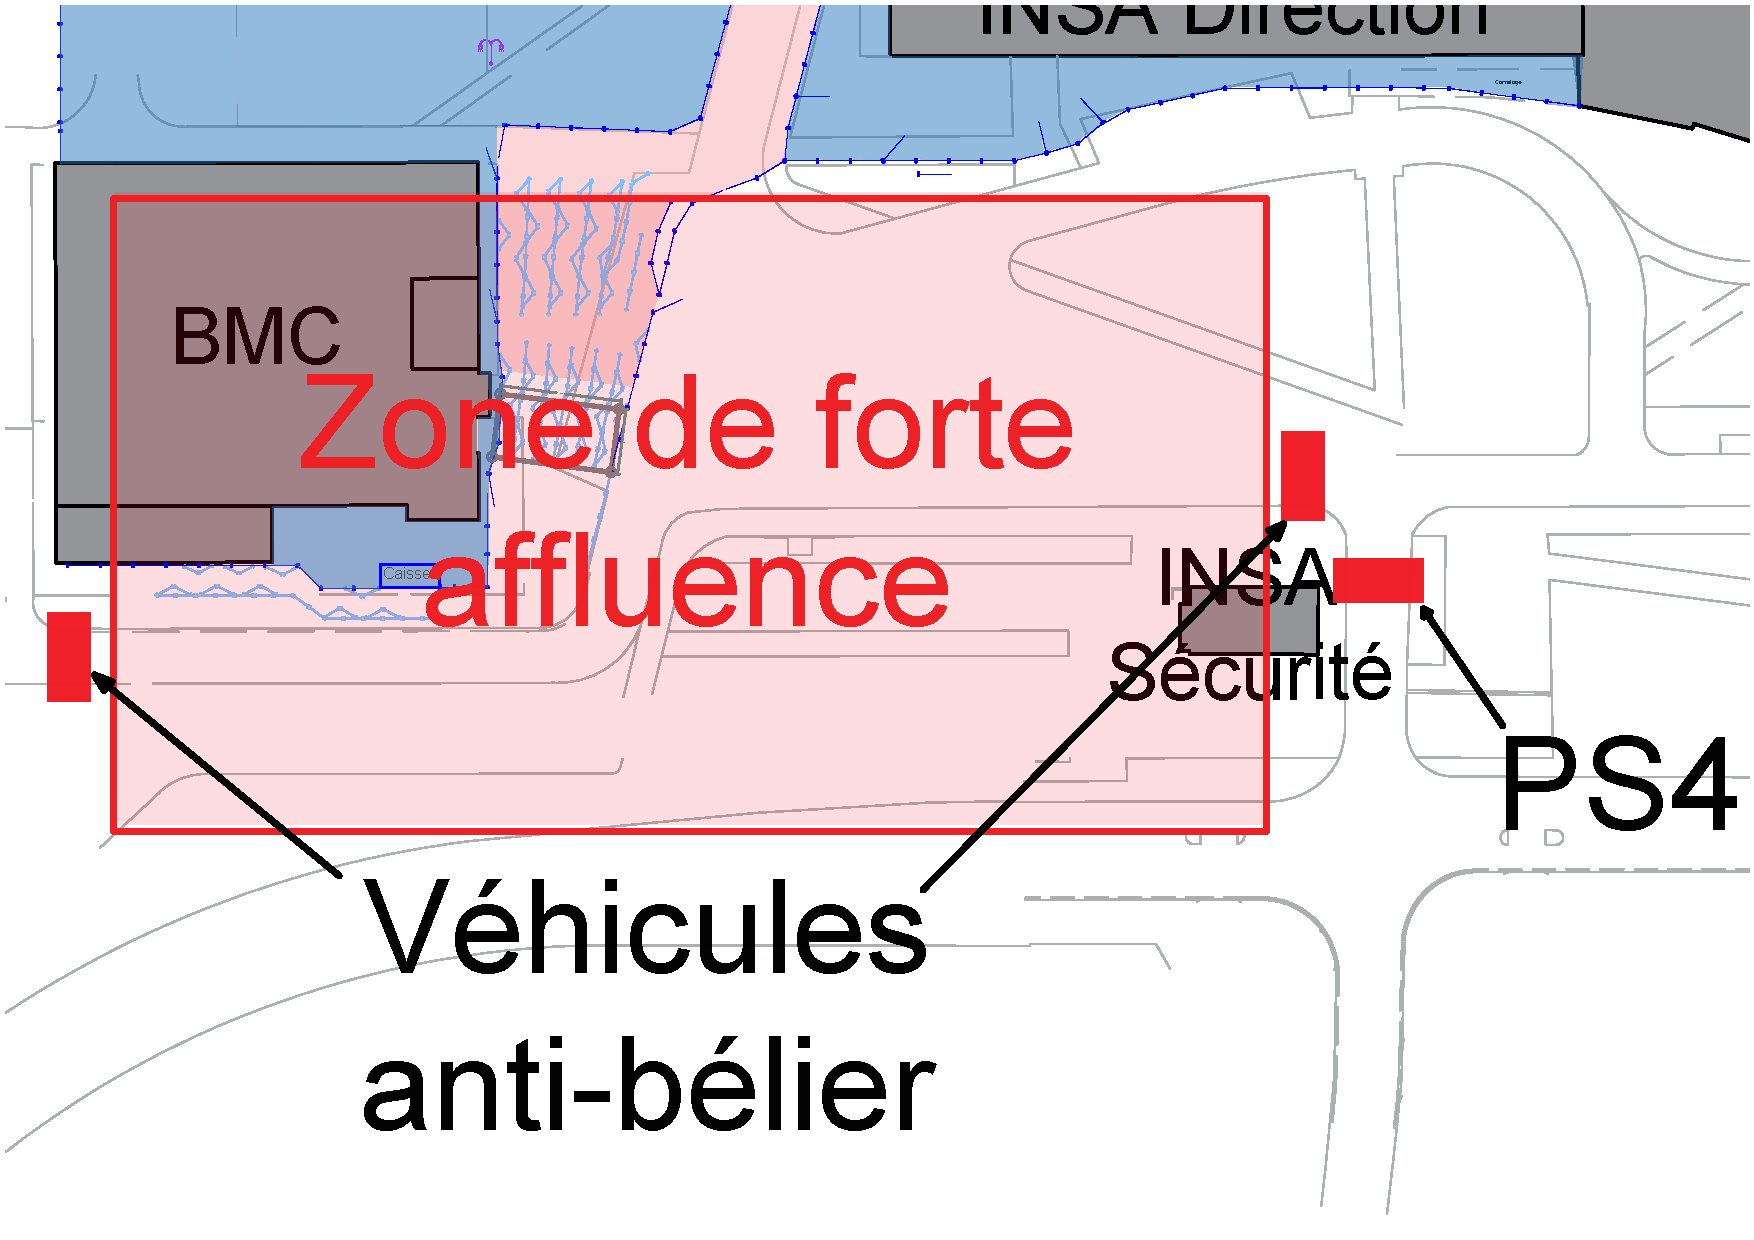
\includegraphics[width=.95\textheight, angle=90]{Exports/Plan_24h_44eme-Vehicules_beliers}\end{center}

\section{Plans quadrillés}
	\begin{center}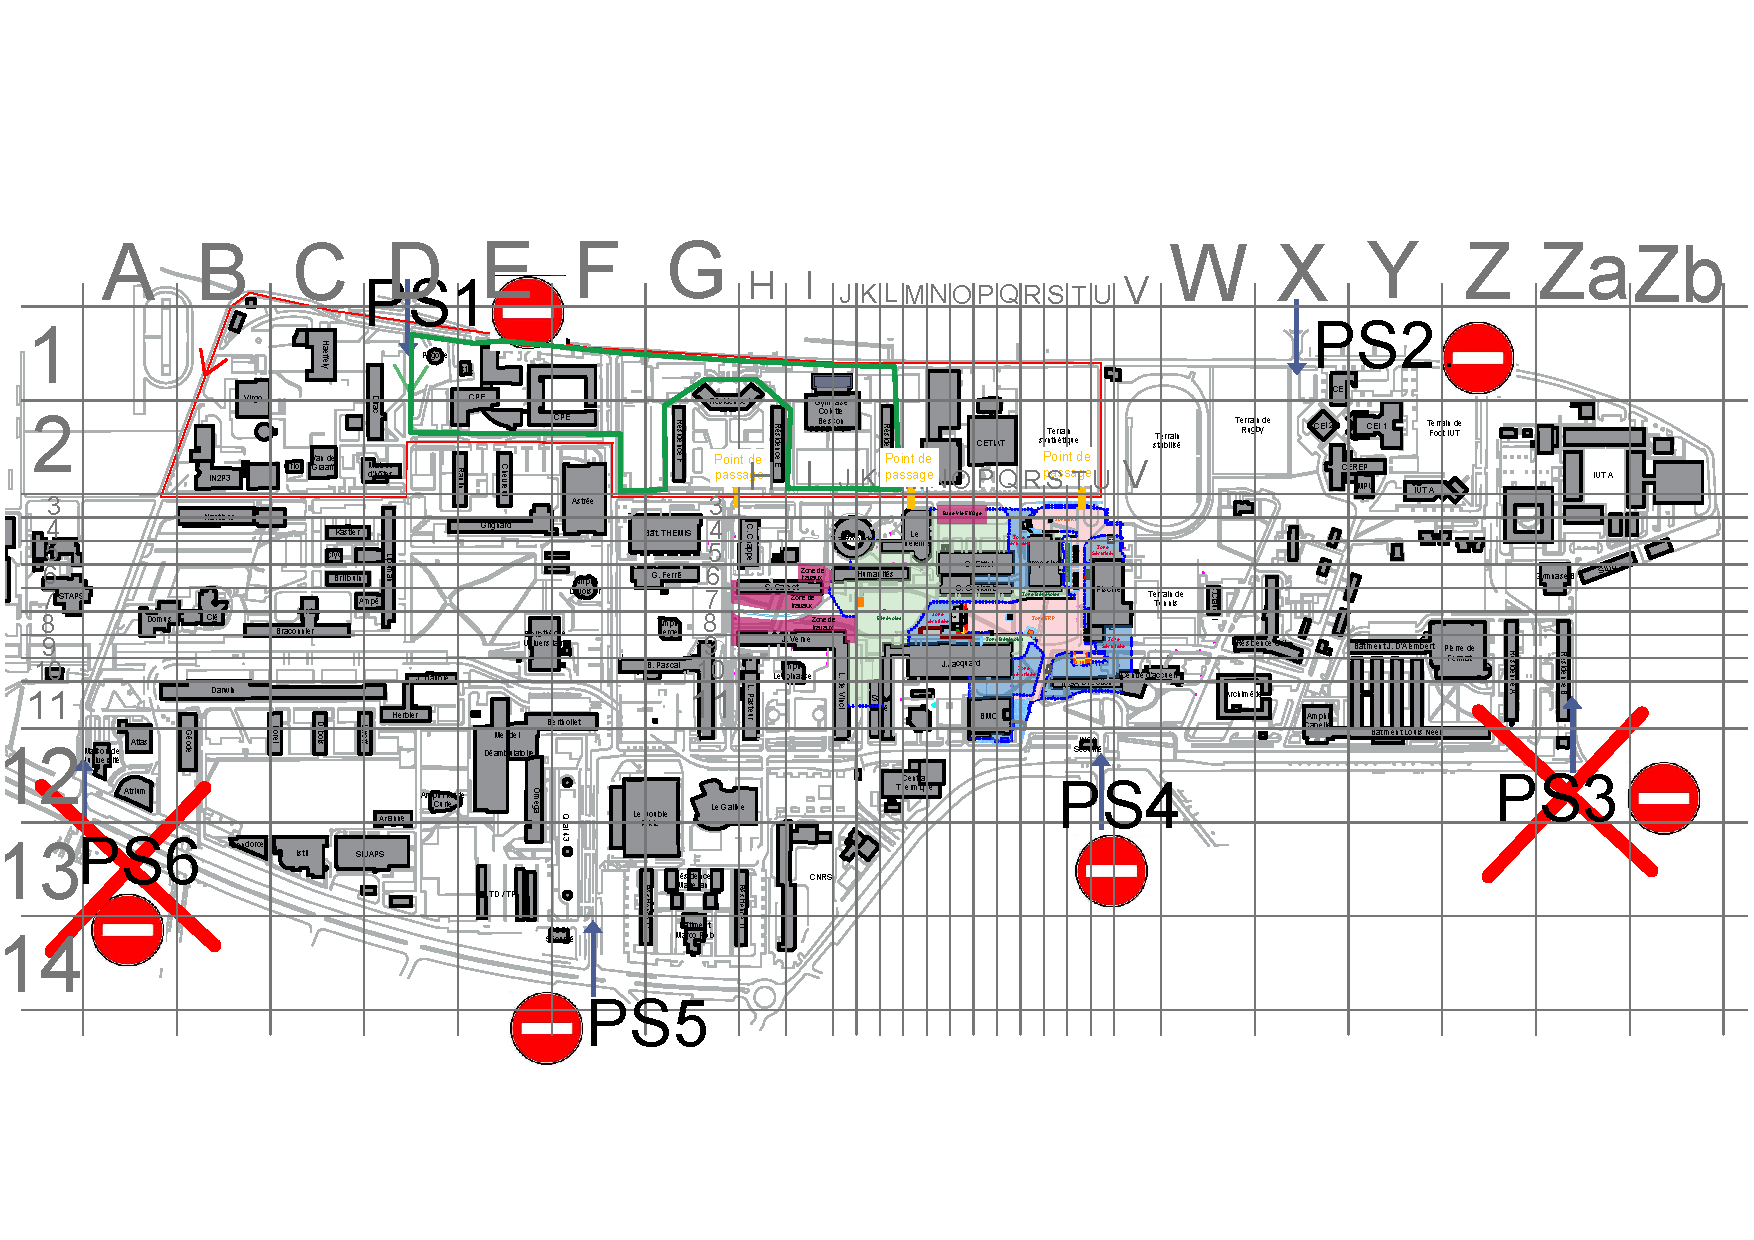
\includegraphics[width=.95\textheight, angle=90]{Exports/Plan_24h_44eme-Quadrillage_campus}\end{center}
	\begin{center}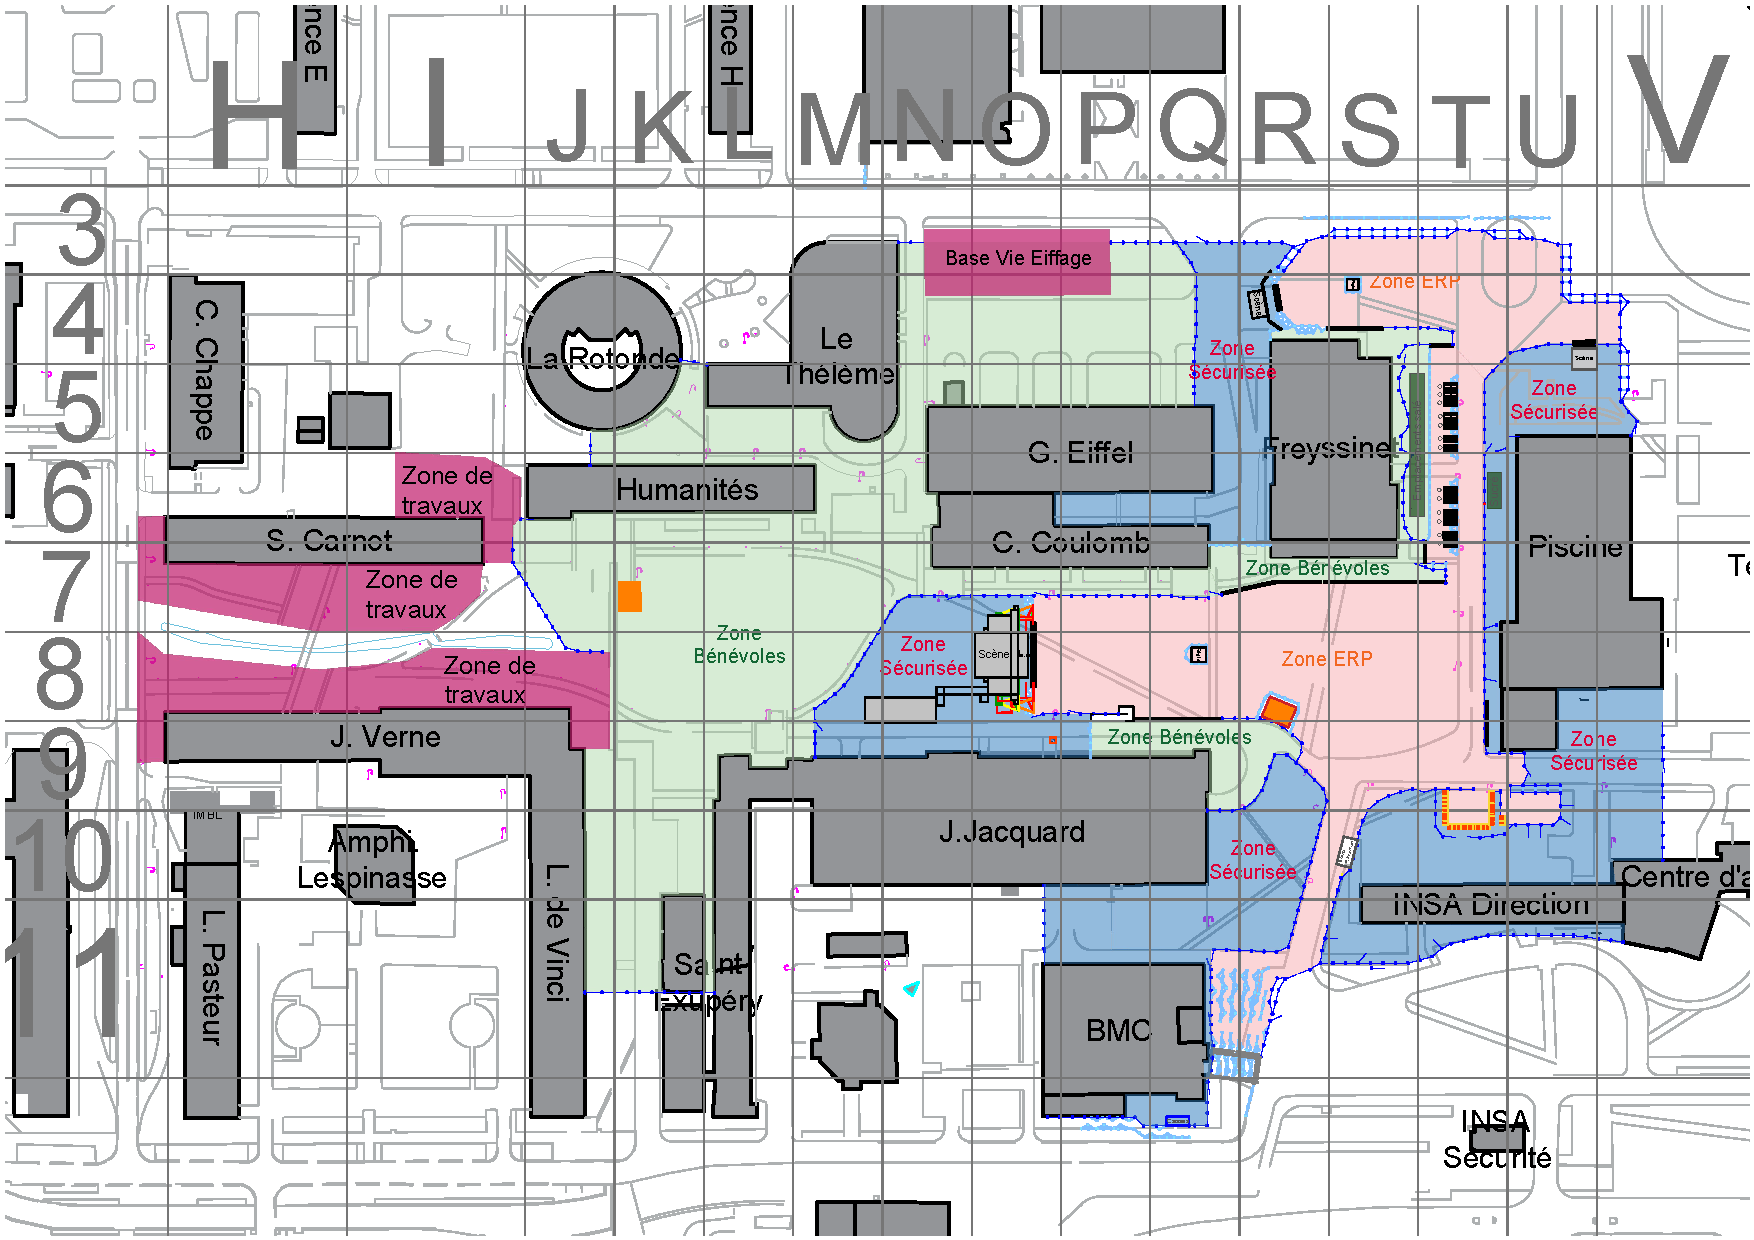
\includegraphics[width=.95\textheight, angle=90]{Exports/Plan_24h_44eme-Quadrillage_zoom}\end{center}
\end{document}